%  A simple AAU report template.
%  2015-05-08 v. 1.2.0
%  Copyright 2010-2015 by Jesper Kjær Nielsen <jkn@es.aau.dk>
%
%  This is free software: you can redistribute it and/or modify
%  it under the terms of the GNU General Public License as published by
%  the Free Software Foundation, either version 3 of the License, or
%  (at your option) any later version.
%
%  This is distributed in the hope that it will be useful,
%  but WITHOUT ANY WARRANTY; without even the implied warranty of
%  MERCHANTABILITY or FITNESS FOR A PARTICULAR PURPOSE.  See the
%  GNU General Public License for more details.
%
%  You can find the GNU General Public License at <http://www.gnu.org/licenses/>.
%
%  A simple AAU report template.
%  2015-05-08 v. 1.2.0
%  Copyright 2010-2015 by Jesper Kjær Nielsen <jkn@es.aau.dk>
%
%  This is free software: you can redistribute it and/or modify
%  it under the terms of the GNU General Public License as published by
%  the Free Software Foundation, either version 3 of the License, or
%  (at your option) any later version.
%
%  This is distributed in the hope that it will be useful,
%  but WITHOUT ANY WARRANTY; without even the implied warranty of
%  MERCHANTABILITY or FITNESS FOR A PARTICULAR PURPOSE.  See the
%  GNU General Public License for more details.
%
%  You can find the GNU General Public License at <http://www.gnu.org/licenses/>.
%
\documentclass[11pt,twoside,a4paper,openright]{report}
%%%%%%%%%%%%%%%%%%%%%%%%%%%%%%%%%%%%%%%%%%%%%%%%
% Language, Encoding and Fonts
% http://en.wikibooks.org/wiki/LaTeX/Internationalization
%%%%%%%%%%%%%%%%%%%%%%%%%%%%%%%%%%%%%%%%%%%%%%%%
% Select encoding of your inputs. Depends on
% your operating system and its default input
% encoding. Typically, you should use
%   Linux  : utf8 (most modern Linux distributions)
%            latin1 
%   Windows: ansinew
%            latin1 (works in most cases)
%   Mac    : applemac
% Notice that you can manually change the input
% encoding of your files by selecting "save as"
% an select the desired input encoding. 
\usepackage[utf8]{inputenc}
% Make latex understand and use the typographic
% rules of the language used in the document.
\usepackage[english]{babel}
% Use the palatino font
\usepackage[sc]{mathpazo}
\linespread{1.05}         % Palatino needs more leading (space between lines)
% Choose the font encoding
\usepackage[T1]{fontenc}
%%%%%%%%%%%%%%%%%%%%%%%%%%%%%%%%%%%%%%%%%%%%%%%%
% Graphics and Tables
% http://en.wikibooks.org/wiki/LaTeX/Importing_Graphics
% http://en.wikibooks.org/wiki/LaTeX/Tables
% http://en.wikibooks.org/wiki/LaTeX/Colors
%%%%%%%%%%%%%%%%%%%%%%%%%%%%%%%%%%%%%%%%%%%%%%%%
% load a colour package
\usepackage{xcolor}
\definecolor{aaublue}{RGB}{33,26,82}% dark blue
% The standard graphics inclusion package
\usepackage{graphicx}
% Set up how figure and table captions are displayed
\usepackage{caption}
\captionsetup{%
  font=footnotesize,% set font size to footnotesize
  labelfont=bf % bold label (e.g., Figure 3.2) font
}
% Make the standard latex tables look so much better
\usepackage{array,booktabs}
% Enable the use of frames around, e.g., theorems
% The framed package is used in the example environment
\usepackage{framed}

%%%%%%%%%%%%%%%%%%%%%%%%%%%%%%%%%%%%%%%%%%%%%%%%
% Mathematics
% http://en.wikibooks.org/wiki/LaTeX/Mathematics
%%%%%%%%%%%%%%%%%%%%%%%%%%%%%%%%%%%%%%%%%%%%%%%%
% Defines new environments such as equation,
% align and split 
\usepackage{amsmath}
% Adds new math symbols
\usepackage{amssymb}
% Use theorems in your document
% The ntheorem package is also used for the example environment
% When using thmmarks, amsmath must be an option as well. Otherwise \eqref doesn't work anymore.
\usepackage[framed,amsmath,thmmarks]{ntheorem}

%%%%%%%%%%%%%%%%%%%%%%%%%%%%%%%%%%%%%%%%%%%%%%%%
% Page Layout
% http://en.wikibooks.org/wiki/LaTeX/Page_Layout
%%%%%%%%%%%%%%%%%%%%%%%%%%%%%%%%%%%%%%%%%%%%%%%%
% Change margins, papersize, etc of the document
\usepackage[
  inner=28mm,% left margin on an odd page
  outer=41mm,% right margin on an odd page
  ]{geometry}
% Modify how \chapter, \section, etc. look
% The titlesec package is very configureable
\usepackage{titlesec}
\titleformat{\chapter}[display]{\normalfont\huge\bfseries}{\chaptertitlename\ \thechapter}{20pt}{\Huge}
\titleformat*{\section}{\normalfont\Large\bfseries}
\titleformat*{\subsection}{\normalfont\large\bfseries}
\titleformat*{\subsubsection}{\normalfont\normalsize\bfseries}
%\titleformat*{\paragraph}{\normalfont\normalsize\bfseries}
%\titleformat*{\subparagraph}{\normalfont\normalsize\bfseries}

% Clear empty pages between chapters
\let\origdoublepage\cleardoublepage
\newcommand{\clearemptydoublepage}{%
  \clearpage
  {\pagestyle{empty}\origdoublepage}%
}
\let\cleardoublepage\clearemptydoublepage

% Change the headers and footers
\usepackage{fancyhdr}
\pagestyle{fancy}
\fancyhf{} %delete everything
\renewcommand{\headrulewidth}{0pt} %remove the horizontal line in the header
\fancyhead[RE]{\small\nouppercase\leftmark} %even page - chapter title
\fancyhead[LO]{\small\nouppercase\rightmark} %uneven page - section title
\fancyhead[LE,RO]{\thepage} %page number on all pages
% Do not stretch the content of a page. Instead,
% insert white space at the bottom of the page
\raggedbottom
% Enable arithmetics with length. Useful when
% typesetting the layout.
\usepackage{calc}

%%%%%%%%%%%%%%%%%%%%%%%%%%%%%%%%%%%%%%%%%%%%%%%%
% Bibliography
% http://en.wikibooks.org/wiki/LaTeX/Bibliography_Management
%%%%%%%%%%%%%%%%%%%%%%%%%%%%%%%%%%%%%%%%%%%%%%%%
%\usepackage[backend=bibtex,
%  bibencoding=utf8
%  ]{biblatex}
%\addbibresource{bib/mybib}

%%%%%%%%%%%%%%%%%%%%%%%%%%%%%%%%%%%%%%%%%%%%%%%%
% Misc
%%%%%%%%%%%%%%%%%%%%%%%%%%%%%%%%%%%%%%%%%%%%%%%%
% Add bibliography and index to the table of
% contents
\usepackage[nottoc]{tocbibind}
% Add the command \pageref{LastPage} which refers to the
% page number of the last page
\usepackage{lastpage}
% Add todo notes in the margin of the document
\usepackage[
%  disable, %turn off todonotes
  colorinlistoftodos, %enable a coloured square in the list of todos
  textwidth=\marginparwidth, %set the width of the todonotes
  textsize=scriptsize, %size of the text in the todonotes
  ]{todonotes}

\usepackage{listings}
\lstset{
language=C,
tabsize=4,
basicstyle=\fontsize{11}{13}\ttfamily\footnotesize,
showspaces=false,
showstringspaces=false,
captionpos=b,
breaklines=true
}

\usepackage{multirow}
\usepackage{float}
\usepackage[caption = false]{subfig}
%%%%%%%%%%%%%%%%%%%%%%%%%%%%%%%%%%%%%%%%%%%%%%%%
% Hyperlinks
% http://en.wikibooks.org/wiki/LaTeX/Hyperlinks
%%%%%%%%%%%%%%%%%%%%%%%%%%%%%%%%%%%%%%%%%%%%%%%%
% Enable hyperlinks and insert info into the pdf
% file. Hypperref should be loaded as one of the 
% last packages
\usepackage{hyperref}
\hypersetup{%
	pdfpagelabels=true,%
	plainpages=false,%
	pdfauthor={Author(s)},%
	pdftitle={Title},%
	pdfsubject={Subject},%
	bookmarksnumbered=true,%
	colorlinks=false,%
	citecolor=black,%
	filecolor=black,%
	linkcolor=black,% you should probably change this to black before printing
	urlcolor=black,%
	pdfstartview=FitH%
}% package inclusion and set up of the document
% see, e.g., http://en.wikibooks.org/wiki/LaTeX/Formatting#Hyphenation
% for more information on word hyphenation
\hyphenation{ex-am-ple hy-phen-a-tion short}
\hyphenation{long la-tex}% 
%  A simple AAU report template.
%  2015-05-08 v. 1.2.0
%  Copyright 2010-2015 by Jesper Kjær Nielsen <jkn@es.aau.dk>
%
%  This is free software: you can redistribute it and/or modify
%  it under the terms of the GNU General Public License as published by
%  the Free Software Foundation, either version 3 of the License, or
%  (at your option) any later version.
%
%  This is distributed in the hope that it will be useful,
%  but WITHOUT ANY WARRANTY; without even the implied warranty of
%  MERCHANTABILITY or FITNESS FOR A PARTICULAR PURPOSE.  See the
%  GNU General Public License for more details.
%
%  You can find the GNU General Public License at <http://www.gnu.org/licenses/>.
%
%
%
% see, e.g., http://en.wikibooks.org/wiki/LaTeX/Customizing_LaTeX#New_commands
% for more information on how to create macros

%%%%%%%%%%%%%%%%%%%%%%%%%%%%%%%%%%%%%%%%%%%%%%%%
% Macros for the titlepage
%%%%%%%%%%%%%%%%%%%%%%%%%%%%%%%%%%%%%%%%%%%%%%%%
%Creates the aau titlepage
\newcommand{\aautitlepage}[3]{%
  {
    %set up various length
    \ifx\titlepageleftcolumnwidth\undefined
      \newlength{\titlepageleftcolumnwidth}
      \newlength{\titlepagerightcolumnwidth}
    \fi
    \setlength{\titlepageleftcolumnwidth}{0.5\textwidth-\tabcolsep}
    \setlength{\titlepagerightcolumnwidth}{\textwidth-2\tabcolsep-\titlepageleftcolumnwidth}
    %create title page
    \thispagestyle{empty}
    \noindent%
    \begin{tabular}{@{}ll@{}}
      \parbox{\titlepageleftcolumnwidth}{
        \iflanguage{danish}{%
          \includegraphics[width=\titlepageleftcolumnwidth]{figures/aau_logo_da}
        }{%
          \includegraphics[width=\titlepageleftcolumnwidth]{figures/aau_logo_en}
        }
      } &
      \parbox{\titlepagerightcolumnwidth}{\raggedleft\sf\small
        #2
      }\bigskip\\
       #1 &
      \parbox[t]{\titlepagerightcolumnwidth}{%
      \textbf{Abstract:}\bigskip\par
        \fbox{\parbox{\titlepagerightcolumnwidth-2\fboxsep-2\fboxrule}{%
          #3
        }}
      }\\
    \end{tabular}
    \vfill
    \iflanguage{danish}{%
      \noindent{\footnotesize\emph{Rapportens indhold er frit tilgængeligt, men offentliggørelse (med kildeangivelse) må kun ske efter aftale med forfatterne.}}
    }{%
      \noindent{\footnotesize\emph{The content of this report is freely available, but publication (with reference) may only be pursued due to agreement with the author.}}
    }
    \clearpage
  }
}

%Create english project info
\newcommand{\englishprojectinfo}[8]{%
  \parbox[t]{\titlepageleftcolumnwidth}{
    \textbf{Title:}\\ #1\bigskip\par
    \textbf{Theme:}\\ #2\bigskip\par
    \textbf{Project Period:}\\ #3\bigskip\par
    \textbf{Project Group:}\\ #4\bigskip\par
    \textbf{Participant(s):}\\ #5\bigskip\par
    \textbf{Supervisor(s):}\\ #6\bigskip\par
    \textbf{Copies:} #7\bigskip\par
    \textbf{Page Numbers:} \pageref{LastPage}\bigskip\par
    \textbf{Date of Completion:}\\ #8
  }
}

%Create danish project info
\newcommand{\danishprojectinfo}[8]{%
  \parbox[t]{\titlepageleftcolumnwidth}{
    \textbf{Titel:}\\ #1\bigskip\par
    \textbf{Tema:}\\ #2\bigskip\par
    \textbf{Projektperiode:}\\ #3\bigskip\par
    \textbf{Projektgruppe:}\\ #4\bigskip\par
    \textbf{Deltager(e):}\\ #5\bigskip\par
    \textbf{Vejleder(e):}\\ #6\bigskip\par
    \textbf{Oplagstal:} #7\bigskip\par
    \textbf{Sidetal:} \pageref{LastPage}\bigskip\par
    \textbf{Afleveringsdato:}\\ #8
  }
}

%%%%%%%%%%%%%%%%%%%%%%%%%%%%%%%%%%%%%%%%%%%%%%%%
% An example environment
%%%%%%%%%%%%%%%%%%%%%%%%%%%%%%%%%%%%%%%%%%%%%%%%
\theoremheaderfont{\normalfont\bfseries}
\theorembodyfont{\normalfont}
\theoremstyle{break}
\def\theoremframecommand{{\color{gray!50}\vrule width 5pt \hspace{5pt}}}
\newshadedtheorem{exa}{Example}[chapter]
\newenvironment{example}[1]{%
		\begin{exa}[#1]
}{%
		\end{exa}
}% my new macros

\begin{document}
%frontmatter
\pagestyle{empty} %disable headers and footers
\pagenumbering{roman} %use roman page numbering in the frontmatter
%  A simple AAU report template.
%  2015-05-08 v. 1.2.0
%  Copyright 2010-2015 by Jesper Kjær Nielsen <jkn@es.aau.dk>
%
%  This is free software: you can redistribute it and/or modify
%  it under the terms of the GNU General Public License as published by
%  the Free Software Foundation, either version 3 of the License, or
%  (at your option) any later version.
%
%  This is distributed in the hope that it will be useful,
%  but WITHOUT ANY WARRANTY; without even the implied warranty of
%  MERCHANTABILITY or FITNESS FOR A PARTICULAR PURPOSE.  See the
%  GNU General Public License for more details.
%
%  You can find the GNU General Public License at <http://www.gnu.org/licenses/>.
%
\pdfbookmark[0]{Front page}{label:frontpage}%
\begin{titlepage}
  \addtolength{\hoffset}{0.5\evensidemargin-0.5\oddsidemargin} %set equal margins on the frontpage - remove this line if you want default margins
  \noindent%
  \begin{tabular}{@{}p{\textwidth}@{}}
    \toprule[2pt]
    \midrule
    \vspace{0.2cm}
    \begin{center}
    \Huge{\textbf{
      Infraestructura básica
    }}
    \end{center}
    \begin{center}
      \Large{
         66:20 Organización de Computadoras
      }
    \end{center}
    \vspace{0.2cm}\\
    \midrule
    \toprule[2pt]
  \end{tabular}
  \vspace{4 cm}
  \begin{center}
    {\large
      Trabajo práctico 0
    }\\
    \vspace{0.6cm}
    {\Large
      Axel Lijdens (95772)\\
      Eduardo R Madariaga (90824)
    }
  \end{center}
  \vfill
  \begin{center}
  Univesidad de Buenos Aires - FIUBA
  \end{center}
\end{titlepage}
\clearpage
%\thispagestyle{empty}
{\small
\strut\vfill % push the content to the bottom of the page
\noindent Copyright \copyright{} Aalborg University 2015\par
\vspace{0.2cm}
\noindent Here you can write something about which tools and software you have used for typesetting the document, running simulations and creating figures. If you do not know what to write, either leave this page blank or have a look at the colophon in some of your books.
}
\clearpage
%\pdfbookmark[0]{English title page}{label:titlepage_en}
\aautitlepage{%
  \englishprojectinfo{
    Project Title %title
  }{%
    Scientific Theme %theme
  }{%
    Fall Semester 2010 %project period
  }{%
    XXX % project group
  }{%
    %list of group members
    Author 1\\ 
    Author 2\\
    Author 3
  }{%
    %list of supervisors
    Supervisor 1\\
    Supervisor 2
  }{%
    1 % number of printed copies
  }{%
    \today % date of completion
  }%
}{%department and address
  \textbf{Electronics and IT}\\
  Aalborg University\\
  \href{http://www.aau.dk}{http://www.aau.dk}
}{% the abstract
  Here is the abstract
}

\cleardoublepage
{\selectlanguage{danish}
\pdfbookmark[0]{Danish title page}{label:titlepage_da}
\aautitlepage{%
  \danishprojectinfo{
    Rapportens titel %title
  }{%
    Semestertema %theme
  }{%
    Efterårssemestret 2010 %project period
  }{%
    XXX % project group
  }{%
    %list of group members
    Forfatter 1\\ 
    Forfatter 2\\
    Forfatter 3
  }{%
    %list of supervisors
    Vejleder 1\\
    Vejleder 2
  }{%
    1 % number of printed copies
  }{%
    \today % date of completion
  }%
}{%department and address
  \textbf{Elektronik og IT}\\
  Aalborg Universitet\\
  \href{http://www.aau.dk}{http://www.aau.dk}
}{% the abstract
  Her er resuméet
}}
\cleardoublepage
\pdfbookmark[0]{Contents}{label:contents}
\pagestyle{fancy} %enable headers and footers again
\tableofcontents
%\listoftodos
\chapter*{Pr\'ologo\markboth{Preface}{Preface}}\label{ch:preface}
\addcontentsline{toc}{chapter}{Pr\'ologo}

\section{Objetivos}

Familiarizarse con las herramientas de software que usaremos en los siguientes trabajos,
implementando un programa y su correspondiente documentación que resuelvan el problema
descripto más abajo.

\section{Alcance}

Este trabajo práctico es de elaboración grupal, evaluación individual, y de carácter obligatorio para todos alumnos del curso.

\section{Requisitos}
El trabajo deber\'a ser entregado personalmente, en la fecha estipulada, con una car\'atula que contenga los datos completos de todos los integrantes.\\

Adem\'as, es necesario que el trabajo pr\'actico incluya, la presentaci\'on de los resultados obtenidos, explicando, cuando corresponda, con fundamentos reales, las causas o razones de cada resultado obtenido.\\

El informe deber\'a respetar el modelo de referencia que se encuentra en el grupo, y se valorar\'an aquellos escritos usando la herramienta TEX / LATEX.

\section{Recursos}

Usaremos el programa GXemul para simular el entorno de desarrollo que utilizaremos en este y otros trabajos prácticos, una máquina MIPS corriendo una versión reciente del sistema operativo NetBSD.
Durante la primera clase del curso presentaremos brevemente los pasos necesarios para la
instalación y configuración del entorno de desarrollo.
\\
\section{Fecha de entrega}

La última fecha de entrega y presentación ser\'a el jueves 5 de abril de 2018.
\\
\section{Informe}\label{informe}
El informe deberá incluir:
\begin{itemize}
\item Documentación relevante al diseño e implementación del programa.
\item Documentación relevante al proceso de compilación: cómo obtener el ejecutable a partir de los archivos fuente.
\item Las corridas de prueba, con los comentarios pertinentes.
\item El código fuente, en lenguaje C.
\item Este enunciado.
\end{itemize}

\cleardoublepage
%mainmatter
\pagenumbering{arabic} %use arabic page numbering in the mainmatter
\chapter{Introducci\'on}\label{ch:introduction}

\section{El comando wc}

El comando de Unix wc toma como entrada un archivo o stdin, y cuenta las palabras, las l\'ineas y la cantidad de caracteres que contiene.

\section{ Programas a desarrollar}
El programa a escribir, en lenguaje C, recibir\'a un nombre de archivo que
contiene texto (o el archivo mismo por stdin) e imprimir\'a por stdout la
cantidad de l\'ineas, palabras y caracteres que contiene, junto con el nombre
del archivo.

\section{Ejemplos}
Primero, usamos la opci\'on -h para ver el mensaje de ayuda:\

\begin{lstlisting}[numbers=left, tabsize=2, basicstyle=\fontsize{11}{13}\ttfamily, frame=single, caption={mensaje de ayuda}]
$ tp0 -h
Usage:
tp0 -h
tp0 -V
tp0 [options] file
Options:
-V, --version Print version and quit.
-h, --help Print this information.
-l, --words Print number of lines in file.
-w, --words Print number of words in file.
-c, --words Print number of characters in file.
-i, --input Path to input file.
Examples:
tp0 -w -i input.txt
Luego, lo usamos con un peque\~no fragmento de texto:
$echo -n "El tractorcito rojo que silbo y bufo" > entrada.txt
$tp0 -w -i entrada.txt
7 entrada.txt
$
\end{lstlisting}

\section{Mediciones}

Se deber\'a medir el tiempo insumido por el programa para el caso de los archivos alice.txt, beowulf.txt, cyclopedia.txt y elquijote.txt. \\

Graficar el tiempo insumido contra el tama\~no de muestra. Se deber\'a comprobar que el programa acepta las opciones dadas, y que reporta un error ante situaciones an\'omalas (como no encontrar el archivo solicitado). La ejecuci\'on del programa debe realizarse bajo el entorno MIPS.

\chapter{Desarrollo}\label{ch:ch2label}

\section{Compilaci\'on}

Para la compilaci\'on del c\'odigo se utilizo un Makefile que se muestra a continuaci\'on:

\begin{tiny}

\begin{lstlisting}[numbers=left, tabsize=2, basicstyle=\fontsize{11}{13}\ttfamily, frame=single, caption={makefile}]
# makefile parameters
BIN_NAME    := tp
SRCDIR      := src
TESTDIR     := tests
BUILDDIR    := int
TARGETDIR   := target
SRCEXT      := c

# compiler parameters
CC          := gcc
CFLAGS      := -O3 -std=c99 -Wall -Wpedantic -Werror
LIB         :=
INC         := /usr/local/include
DEFINES     :=


#-----------------------------------------------
# DO NOT EDIT BELOW THIS LINE
#-----------------------------------------------

# binaries file names
# each binary source code is expected to be in $(SRCDIR)/<binary>
TARGET := $(TARGETDIR)/$(BIN_NAME)

# sets the src directory in the VPATH
VPATH := $(SRCDIR)

# sets the build directory based on the binary
BUILDDIR := $(BUILDDIR)

# source files
SRCS := $(shell find $(SRCDIR) -type f -name *.$(SRCEXT))

# object files
OBJS := $(patsubst %,$(BUILDDIR)/$(BIN_NAME)/%,$(SRCS:.$(SRCEXT)=.o))

# includes the flag to generate the dependency files when compiling
CFLAGS += -MD


# special definitions used for the unit tests
ifeq ($(MAKECMDGOALS),tests)
    # adds an extra include so the tests can include the sources
	INC += src

	# sets the special define for tests
	DEFINES := __TESTS__ $(DEFINES)

	# includes the tests directory in the VPATH
	VPATH := $(TESTDIR) $(VPATH)

	# test sources
	TEST_SRCS := $(shell find $(TESTDIR) -type f -name *.$(SRCEXT))

	# test objects
	OBJS := $(patsubst $(BUILDDIR)/$(BIN_NAME)/%,$(BUILDDIR)/tests/%,$(OBJS))
	OBJS := $(patsubst %,$(BUILDDIR)/tests/%,$(TEST_SRCS:.$(SRCEXT)=.o)) $(OBJS)
endif

# adds the include prefix to the include directories
INC := $(addprefix -I,$(INC))

# adds the lib prefix to the libraries
LIB := $(addprefix -l,$(LIB))

# adds the define prefix to the defines
DEFINES := $(addprefix -D,$(DEFINES))


# builds the binary
$(TARGET): $(OBJS) | dirs
	@$(CC) $(CFLAGS) $(INC) $(DEFINES) $^ $(LIB) -o $@
	@echo "LD $@"

# compiles the tests
tests: $(TARGET) | dirs
	python tests/run.py $(TARGET)

# shows usage
help:
	@echo "Para compilar el binario:"
	@echo
	@echo "\t\033[1;92m$$ make\033[0m"
	@echo
	@echo "Para compilar y ejecutar las pruebas (require python 2.7+ instalado):"
	@echo
	@echo "\t\033[1;92m$$ make tests\033[0m"
	@echo
	@echo "Los binarios compilados se encuentran en \033[1;92m$(TARGETDIR)\033[0m."
	@echo

# clean objects and binaries
clean:
	@$(RM) -rf $(BUILDDIR) $(TARGETDIR)

# creates the directories
dirs:
	@mkdir -p $(TARGETDIR)
	@mkdir -p $(BUILDDIR)

# rule to build object files
$(BUILDDIR)/$(BIN_NAME)/%.o $(BUILDDIR)/tests/%.o: %.$(SRCEXT)
	@mkdir -p $(basename $@)
	@echo "CC $<"
	@$(CC) $(CFLAGS) $(INC) $(DEFINES) $(LIB) -c -o $@ $<


.PHONY: clean dirs tests

# includes generated dependency files
-include $(OBJS:.o=.d)
\end{lstlisting}

\end{tiny}

Para la compilaci\'on del c\'odigo basta con ejecutar el Makefile:

\begin{lstlisting}
$ make 
\end{lstlisting}

\section{Corridas de prueba}

A la hora de ejecutar las pruebas, basta usar el mismo Makefile pero ahora con lo opci'on \textbf{tests}:

\begin{lstlisting}
$ make tests
\end{lstlisting}

\subsection{Resultados}

Se utilizaron los 4 archivos de palabras provistos, con los siguientes tama\~nos (en MiB):

\begin{center}

 \begin{tabular}{|c | c|} 
 \hline
  & Size  \\ 
 \hline\hline
Alice & 0.17 \\
\hline
Beowul/f & 0.21 \\
\hline
Cyclopedia & 0.63  \\
\hline
El quijote & 2.1 \\
 \hline
\end{tabular}\\
\end{center}

En la siguiente tabla se muestran los timpos (en segundos) que se tard\'o en ejecutar el programa con cada entrada:

\begin{center}
 \begin{tabular}{|c | c c c c|} 
 \hline
  & Count Bytes & Count Chars & Count words & Count lines \\
 \hline\hline
Alice  & 0.082 & 0.102 & 0.113 & 0.066 \\
\hline
Beowul/f & 0.113 & 0.133 & 0.125 & 0.102 \\
\hline
Cyclopedia  & 0.25 & 0.348 & 0.301 & 0.234 \\
\hline
El quijote & 0.816 & 1.133 & 1 & 0.75 \\
 \hline
\end{tabular}

\end{center}

En base a estos resultados se pueden realizar gr\'aficos para evidenciar la tendencia como se muestran en \ref{some example}

\begin{figure}
\subfloat[]{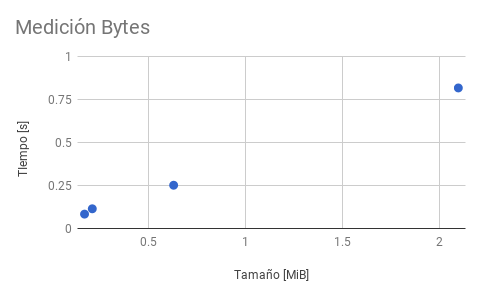
\includegraphics[width = 3in]{figures/chart(0).png}} 
\subfloat[]{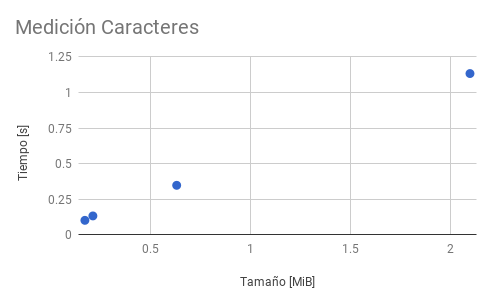
\includegraphics[width = 3in]{figures/chart(1).png}}\\
\subfloat[]{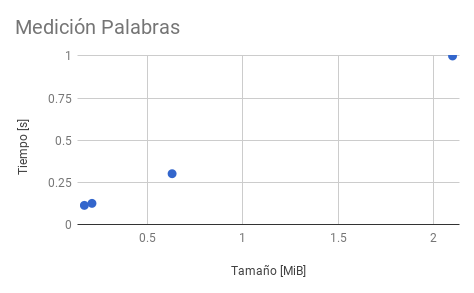
\includegraphics[width = 3in]{figures/chart(2).png}}
\subfloat[]{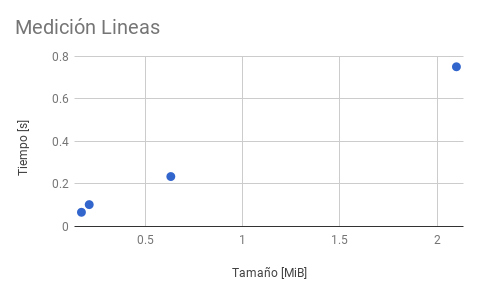
\includegraphics[width = 3in]{figures/chart(3).png}} 
\caption{Gr\'aficos de resultados obtenidos para cada valor de entrada}
\label{some example}
\end{figure}

\subsection{Resultados utilizando MIPS}

Utilizando la m\'aquina virtual, se obtuvieron las mediciones de tiempo utilizando la utilidad \textbf{time}. Los resultados se muestran en la tabla \ref{mipsresult}.


\begin{table}[]
\centering
\caption{My caption}
\label{my-label}
\begin{tabular}{l|l|l|l|l|l|}
\cline{2-6}
                                                  & Count Type & count   & real     & user     & sys      \\ \hline \hline
\multicolumn{1}{|c|}{\multirow{4}{*}{Alice}}      & Bytes      & 177428  & 0m0.082s & 0m0.066s & 0m0.016s \\ \cline{2-6} 
\multicolumn{1}{|c|}{}                            & Chars      & 177412  & 0m0.102  & 0m0.098s & 0m0.004s \\ \cline{2-6} 
\multicolumn{1}{|c|}{}                            & Words      & 30357   & 0m0.113s & 0m0.066s & 0m0.035s \\ \cline{2-6} 
\multicolumn{1}{|c|}{}                            & Lines      & 4046    & 0m0.066s & 0m0.066s & 0m0.000s \\ \hline
\multicolumn{1}{|c|}{\multirow{4}{*}{Beowulf}}    & Bytes      & 224839  & 0m0.113s & 0m0.086s & 0m0.027s \\ \cline{2-6} 
\multicolumn{1}{|c|}{}                            & Chars      & 224806  & 0m0.133s & 0m0.113s & 0m0.020s \\ \cline{2-6} 
\multicolumn{1}{|c|}{}                            & Words      & 37048   & 0m0.125s & 0m0.121s & 0m0.004s \\ \cline{2-6} 
\multicolumn{1}{|c|}{}                            & Lines      & 4562    & 0m0.102s & 0m0.082s & 0m0.020s \\ \hline
\multicolumn{1}{|l|}{\multirow{4}{*}{Cyclopedia}} & Bytes      & 658543  & 0m0.250s & 0m0.242s & 0m0.008s \\ \cline{2-6} 
\multicolumn{1}{|l|}{}                            & Chars      & 658543  & 0m0.348s & 0m0.332s & 0m0.016s \\ \cline{2-6} 
\multicolumn{1}{|l|}{}                            & Words      & 105582  & 0m0.301s & 0m0.293s & 0m0.008s \\ \cline{2-6} 
\multicolumn{1}{|l|}{}                            & Lines      & 17926   & 0m0.234s & 0m0.223s & 0m0.012s \\ \hline
\multicolumn{1}{|l|}{\multirow{4}{*}{El Quijote}} & Bytes      & 2198907 & 0m0.816s & 0m0.789s & 0m0.027s \\ \cline{2-6} 
\multicolumn{1}{|l|}{}                            & Chars      & 2155340 & 0m1.133s & 0m1.094s & 0m0.020s \\ \cline{2-6} 
\multicolumn{1}{|l|}{}                            & Words      & 389470  & 0m1.000s & 0m0.980s & 0m0.020s \\ \cline{2-6} 
\multicolumn{1}{|l|}{}                            & Lines      & 37862   & 0m0.750s & 0m0.734s & 0m0.016s \\ \hline
\end{tabular}
\end{table}

\section{C\'odigo Fuente}


A contiunaci\'on se muestra el c\'odigo fuente:

\begin{tiny}
\begin{lstlisting}[numbers=left, tabsize=2, basicstyle=\fontsize{11}{13}\ttfamily, frame=single, caption={c\'odigo fuente del programa}]
#include <ctype.h>
#include <getopt.h>
#include <inttypes.h>
#include <stdbool.h>
#include <stddef.h>
#include <stdint.h>
#include <stdio.h>
#include <stdlib.h>
#include <string.h>
#include <unistd.h>

/** Tipos de datos */

/** Tipo de contador para los datos de entrada */
typedef enum {
  /** Cuenta los bytes */
  counter_type_byte,

  /** Cuenta los caracteres (teniendo en cuenta los multi-bytes) */
  counter_type_char,

  /** Cuenta las palabras (delimitadas por 'isspace') */
  counter_type_word,

  /** Cuenta las lineas (delimitadas por '\n') */
  counter_type_line,

  /** Valor cuando no se especifico nungun contador. */
  counter_type_invalid,

} counter_type_t;

/** Parametros parseados de la linea de comandos. */
struct args {
  /* el tipo de contador a utilizar para los datos de entrada. */
  counter_type_t counter_type;

  /* Path del archivo con los datos de entrada */
  const char *path;

  /* Boolean indica si se usa stdin */
  bool is_stdin;
};

/** Estructuras de datos */

/** Estructura que uitliza getopt_log para parsear los argumentos de linea de
 * comandos. */
static const struct option _long_opts[] = {
    {.name = "help", .has_arg = no_argument, .flag = NULL, .val = 'h'},
    {.name = "version", .has_arg = no_argument, .flag = NULL, .val = 'V'},
    {.name = "bytes", .has_arg = no_argument, .flag = NULL, .val = 'b'},
    {.name = "chars", .has_arg = no_argument, .flag = NULL, .val = 'c'},
    {.name = "words", .has_arg = no_argument, .flag = NULL, .val = 'w'},
    {.name = "lines", .has_arg = no_argument, .flag = NULL, .val = 'l'},
    {.name = "input", .has_arg = required_argument, .flag = NULL, .val = 'i'},
    {0},
};

/** Funciones */

/**
 * @brief Imprime un mensaje de ayuda y termina el programa.
 *
 * @param bin_name argv[0].
 */
static void _print_help(const char *bin_name) {
  printf("USE: %s [OPTIONS]\n", bin_name);
  printf("Valid options:\n");
  printf("  -h, --help        Prints this message and exits.\n");
  printf("  -V, --version     Prints version and exits.\n");
  printf("  -b, --bytes       Counts input file's bytes and exits.\n");
  printf("  -c, --chars       Counts input file's characters and exits.\n");
  printf("  -w, --words       Counts input file's words and exits.\n");
  printf("  -l, --lines       Counts input file's lines and exits.\n");
  printf(
      "  -i, --input [FILE] means the input will follow the path after -i, if "
      "it is inexistant, stdio will be used.\n");
  printf("\n");
  printf(
      "FILE is the name of the file to read, o '-' to read from "
      "STDIN.\n");
}

/**
 * @brief Imprime la version del programa y termina.
 *
 * @param bin_name argv[0].
 */
static void _print_version(const char *bin_name) {
  printf("%s, version 1.00\n", bin_name);
}

/**
 * @brief Realiza el parseo de los parametros de linea de comandos.
 *
 * @param args Estructura que contiene los parametros parseados.
 * @param argc
 * @param argv
 */
static void _arg_parse(struct args *args, int argc, const char **argv) {
  counter_type_t type = counter_type_invalid;
  args->is_stdin = true;
  int ch = -1;

  while ((ch = getopt_long(argc, (char **)argv, "hVbcwli:", _long_opts, NULL)) != -1) {
    switch (ch) {
      case 'h':
        _print_help(argv[0]);
        exit(0);
        break;

      case 'V':
        _print_version(argv[0]);
        exit(0);
        break;

      case 'b':
        type = counter_type_byte;
        break;

      case 'c':
        type = counter_type_char;
        break;

      case 'w':
        type = counter_type_word;
        break;

      case 'l':
        type = counter_type_line;
        break;

      case 'i':
        args->path = argv[optind - 1];
        args->is_stdin = (strcmp("-", args->path) == 0);
        break;

      /* this is returned when a required argument was not provided */
      case ':':
      case '?':
        exit(1);
    }
  }

  if (type == counter_type_invalid) {
    printf("Counter not specified.\n");
    exit(1);
  }

  /* llena la estructura de salida */
  args->counter_type = type;
}

/**
 * @brief Lee del `input` hasta que no haya mas datos y aplica el contador
 * especificado.
 *
 * @param input Archivo de donde leer los datos.
 * @param counter_type Tipo de contador a utilizar.
 * @return Resultado del contador.
 */
static uint64_t _process_input(FILE *input, counter_type_t counter_type) {
  unsigned int counter = 0;
  char buffer[2048];
  size_t buffer_len = 0;
  char new_byte, prev_byte = 0;

  while (buffer_len = fread(buffer, 1, sizeof(buffer), input), buffer_len > 0) {
    for (size_t i = 0; i < buffer_len; i++) {
      new_byte = buffer[i];
      switch (counter_type) {
        case counter_type_byte:
          counter++;
          break;

        case counter_type_char:
          counter += (new_byte & 0xc0) != 0x80;
          break;

        case counter_type_word:
          if (prev_byte == 0 || (isspace(prev_byte) && !isspace(new_byte))) {
            counter++;
          }
          break;

        case counter_type_line:
          if (new_byte == '\n') {
            counter++;
          }
          break;

        case counter_type_invalid:
          return 0;
      }

      prev_byte = new_byte;
    }
  }

  return counter;
}

int main(int argc, const char *argv[]) {
  struct args args = {0};

  /* parsea la linea de comandos */
  _arg_parse(&args, argc, argv);

  /* Si es STDin, pone el archivo como stdin. Si no abrimos con la ruta */
  FILE *file;

  if (args.is_stdin) {
    file = stdin;
  } else {
    file = fopen(args.path, "r");
    if (file == 0) {
      perror("Error");
      exit(0);
    }
  }

  /* procesa la entrada */
  uint64_t count = _process_input(file, args.counter_type);
  printf("%" PRIu64 "\n", count);

  fclose(file);
  return EXIT_SUCCESS;
}
\end{lstlisting}
\end{tiny}
%\chapter{Conclusion}\label{ch:conclusion}
In case you have questions, comments, suggestions or have found a bug, please do not hesitate to contact me. You can find my contact details below.
  \begin{center}
    Jesper Kjær Nielsen\\
    \href{mailto: jkn@es.aau.dk}{jkn@es.aau.dk}\\
    \href{http://kom.aau.dk/~jkn}{http://kom.aau.dk/\textasciitilde jkn}\\
    Fredrik Bajers Vej 7\\
    9220 Aalborg Ø
  \end{center}
%\printbibliography[heading=bibintoc]
%\label{bib:mybiblio}
%\appendix
%\chapter{Appendix A name}\label{ch:appAlabel}
Here is the first appendix
\end{document}